\documentclass[11pt,a4j]{jreport}

\usepackage{comment}
\usepackage{float}
\usepackage{color}
\usepackage{multicol}
\usepackage{multirow}
\usepackage[dvipdfmx]{pict2e}
\usepackage{wrapfig}
\usepackage{graphicx}
\usepackage{bm}
\usepackage{url}
\usepackage{underscore}
\usepackage{colortbl}
\usepackage{tabularx}
\usepackage{fancyhdr}
\usepackage{ulem}
\usepackage{cite}
\usepackage{amsmath,amssymb,amsfonts}
\usepackage{algorithmic}
\usepackage{textcomp}
\usepackage{xcolor}
\usepackage[ipaex]{pxchfon}
\usepackage{pdfpages}
\usepackage{subcaption}
\usepackage{array}
\usepackage{adjustbox}
\usepackage{lipsum}

\usepackage[number-unit-product=~]{siunitx}

\usepackage[top=30truemm,bottom=30truemm,left=25truemm,right=25truemm]{geometry}

\renewcommand{\arraystretch}{1.2}

\begin{document}

\chapter{はじめに}
%=====================================================================

\section{背景} %1.1
本研究は反射音の到来方向が演奏者に与える影響について検討を行うものであり、コンサートホール音響学の中でも特に演奏者の立場からホールの評価を行うことを試みるステージ音響学の分野に位置づく。研究の前史として、まずコンサートホールの起源とその研究の起こりについて概観する。

\subsection*{コンサートホールの起源}
18世紀以前のヨーロッパにおいて音楽家は主に王室や貴族、教会の保護下で活動していたが、18世紀後半になるとブルジョワジーと呼ばれる中産階級が社会の富と実験を握り始めたことで従来の庇護者の力が相対的に弱まり、市民層を対象としたコンサートにより収入を得る音楽家が現れたとされる。

最初期のコンサートホールは既存の建物を利用したものだったが、市民向けコンサートが興行的な成功を収めるようになると、より多くの聴衆を収容する必要性が高まり、コンサート用の会場として約800席の座席数を持つハノーヴァー・スクエア・ルームズ(1774年)などが建設されるようになった。19世紀以降には2000席程度の座席数を誇るようなより大規模なコンサート専用ホールがヨーロッパ各地に建設されるようになり、特に代表的な初期の大規模コンサートホールとして、ウィーン楽友協会大ホール (1870)、初代ベルリン・フィルハーモニー (1882)、アムステルダムのコンセルトヘボウ (1888)が挙げられる。ルネサンス期に成立したオペラのための大規模な劇場は18世紀にはヨーロッパ各地に建造されていたことを思うと、コンサートホールの歴史は比較的新しいものと言えよう。

\vspace{1\baselineskip}

\begin{figure}[H]
  \begin{minipage}[t]{0.5\linewidth}
    \centering
    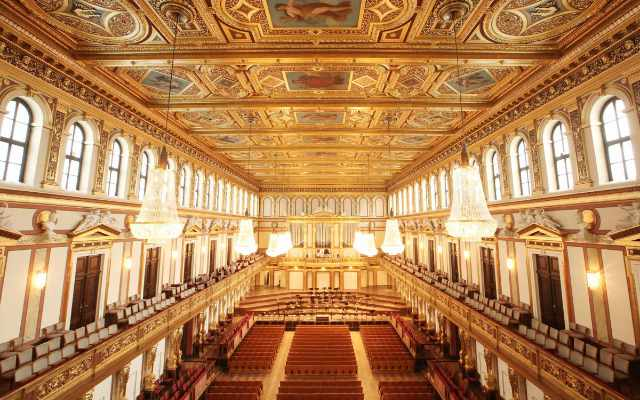
\includegraphics[width=0.9\linewidth]{images/pictureCitation/resized/musikverein.jpg}
    \caption{ウィーン楽友協会大ホール}
    \footnotesize © Wolf-Dieter Grabner, ウィーン楽友協会\\公式ホームページ \cite{musikverein}
    \label{fig:ウィーン楽友協会大ホール}
  \end{minipage}%
  \begin{minipage}[t]{0.5\linewidth}
    \centering
    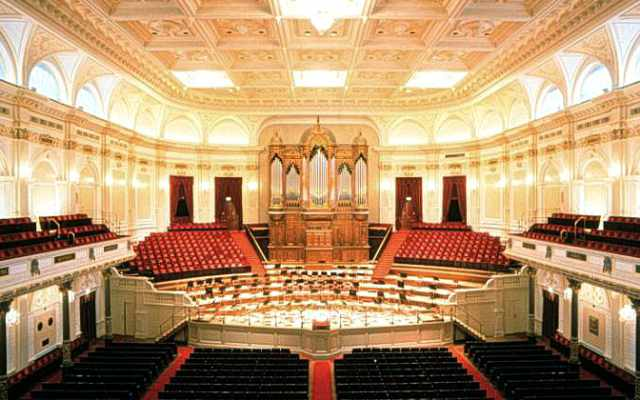
\includegraphics[width=0.9\linewidth]{images/pictureCitation/resized/Concertgebouw.jpg}
    \caption{アムステルダム コンセルトヘボウ}
    \label{fig:コンセルトヘボウ}
    \footnotesize © Amsterdam Municipal Department for the\\ Preservation and Restoration of Historic\\ Buildings and Sites (bMA) \cite{Concertgebouw}
  \end{minipage}
\end{figure}

%=====================================================================

\newpage
\subsection*{コンサートホール音響学の創始}

これらのホールは靴箱のような直方体の空間形状からシューボックス型と呼ばれる形式で、この形状がコンサートホールの形として良いのではないかということは経験的に認識されていたという。特にウィーン楽友協会大ホールは響きの優れたホールとしても有名であるが、しかし、これらのホールの響きは必ずしも音響設計によって狙った響きが実現されたものではない。コンサートホールの建造にあたっての本格的な音響設計の開始は、ボストンシンフォニーホールの設計におけるSabineの音響コンサルティングを待つことになる\cite{清水寧2023}。

Sabineはハーバード大学の物理学の研究者であり、彼の建築音響に関する研究はハーバード大学に建設された Fogg Art Museum (1895)の講義室に生じた「残響により言葉が明瞭に聞こえない」という音響的な問題の改善を依頼されたことから始まった。この問題の解決のための過程でSabineが導入した残響時間や吸音率といった概念は現代の室内音響学の基礎となっており、ボストンシンフォニーホールの音響設計においてもこれらの概念を活用して設計が進められた。これらのSabineの取り組みにより、建築音響工学、そしてコンサートホール音響学が創始された\cite{sabine2005}。それ以降、優れた音響空間をいかにして建築するかという課題に向かって、基本的な残響感から極めて感性的な判断である音の好みに至るまで、物理的あるいは聴覚心理的視点から数多くの研究が積み重ねられてきた。

\vspace{\stretch{1}}

\begin{figure}[H]
  \centering
  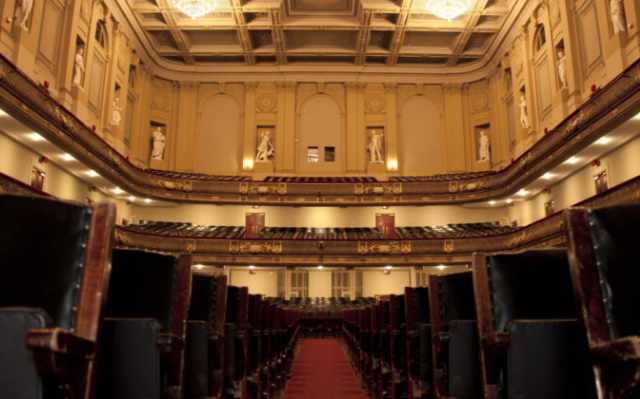
\includegraphics[width=.45\linewidth]{images/pictureCitation/resized/bostonSymphony.jpg}
  \caption{ボストン シンフォニーホール}
  \label{fig:ボストンシンフォニーホール}
  \footnotesize ボストンシンフォニーホール公式ホームページより \cite{bostonSymphony}
\end{figure}

\vspace{\stretch{1}}

%=====================================================================
\newpage
\section{既往研究}

\subsection*{ステージ音響学の始まり}
演奏者にとっても空間の響きが極めて重要であることは演奏者にとっては半ば自明であって、ホール設計者や音響学の研究者にもよく知られていたのではないかと推測されるが、コンサートホール音響学に関する研究は、主に客席での聴こえ方、すなわち聴衆の視点に立って行われてきた。演奏者の視点に立ったコンサートホールに関する音響学の研究領域は今日では「ステージ音響学」と呼ばれて分類されるが、この研究が本格的に行われるようになるのは1970年代に入ってからのことである。

ステージ音響の研究がSabineによるコンサートホール音響学の創始から随分と遅れて始まった理由を直接述べることは困難であるが、「演奏家はホールを評価するというよりも、どうしたらそのホールで良い演奏ができるかということを考える」という言葉\cite{橘1997}によく表れてように、熟練した演奏者であれば空間の響きに合わせて演奏を適応させるべきであると他ならぬ演奏者自身が考えているであろうという動機の点は一つの理由として考えられる。またこのような適応的な演奏の変化を行うという事実から、多数の演奏者を対象として信頼性の高い均一な主観評価結果を得るのが難しいという研究上の困難さがある点も、その理由の一部ではないかと推測できる。
  
ともかくコンサートホール音響学の創始から遅れつつも1970年代にステージ音響に関する研究は始まり、その初期の研究は、模擬音場での演奏実験によって\cite{marhsall1978, nakayama1984, naylor1988}、または実際のホールステージの現場での実験によって\cite{Gade1989II, chiang2003, jeon2005}、音場に対する演奏者の主観印象の評価を求めるものであった。

さらに、菅\cite{suga1986}は演奏者が好むステージ音響状態を説明する指標として「響きの量」「響きの質」「自分の音の出しやすさ」「自分の音の聞き取りやすさ」「他の演奏の聞き取りやすさ」「音の鳴りの手応え」「弱音の伸び」「音の通り」のそれぞれの関係を検討している。その結果、ホールの音響的印象は響きの量・質、自分の音の出しやすさ、聞き取りやすさの四要因の評価でほとんど決定されること、演奏のしやすさの評価はこのうち前三者との相関が高く、これらが音響的総合印象を支配する要因であるとしている。

舞台音響特性の物理的な測定を通した大規模な調査は1989年にGade\cite{Gade1989II}によって初めて行われ、演奏者自身の演奏のしやすさに関する物理指標値として”SUPPORT(ST)”、アンサンブルの取りやすさに関する指標値として”Early Ensemble Level(EEL)”が定義された。また、指揮者、歌手、オーケストラ団員に対するインタビューを通し、演奏家のホールに対する評価項目を響き(Reverberance)、自分の音の聞きやすさ(Support)、音色(Timbre)、ダイナミクス(Dynamics)、互いの音の聞きやすさ(Hearing Each Other)、時差(Time Delay)の六つにまとめている。これらGadeの取り組みの成果がステージ音響学が本格化する画期となったと考えられ、今日ISO3382-1:2009にもSTおよびEELが規格化されており、音響設計やステージ音場の評価に用いられている。なお、ステージ音響指標STに関する説明について、またGadeの提案からISOに規格化されるまでのステージ音響指標値に関する研究の経緯については第2章第1節にて詳細に記述する。

\newpage
\subsection*{ステージ音響学の発展}

菅ら\cite{suga1995}はボストン交響楽団、ライプツィヒ・ゲヴァンドハウス管弦楽団、新日本フィルハーモニー交響楽団の団員に対して多数のホールでのコンサートに基づく主観評価調査を行った結果からホールの音響設計という観点から考慮すべき点について考察し、「舞台の大きさ」「舞台音響反射板の開き具合」「舞台音響反射板の拡散性」という三点をまとめている。

上野ら\cite{Ueno2003a}は、演奏家のホールに対する心象が演奏という能動的行為における個々の意識に密接に関係するものであるため、ホールに対する演奏家の意識の理解のために、実験により検証可能な仮説を設定して統計的にその妥当性を確かめる一般的な心理統計的手法を適用することが難しいという問題を指摘した上で、ホールの音響効果に関する演奏家の言語構造について検討を行い、その結果として、演奏中の演奏家の意識に関して「個人」「共演者」「聴衆」の三つの軸を想定することにより演奏家の言語表現が整理された。

上野らはさらに、演奏者がホール音場についてどのように考えているかについて、演奏者自身の言葉を用いて個人別の評価項目を作成して評価を行う"個別尺度法"を適用した主観評価実験を行い、各演奏家の好みなど総合的な評価に関しては個人差が大きく表れるのに対し、具体的な響きの特徴や音の聴こえ方については複数の演奏家がある程度共通した判断を行っていることを報告している\cite{Ueno2003a}。


\subsection*{ステージへの反射音の到来方向に関する研究}
Gadeにより提案され、今日ではISOに規格化されるステージ音響指標STおよびEELは、舞台上に音源・受音点を置いて測定したインパルス応答において、直接音のエネルギーに対する反射音のエネルギーの量を評価することで、演奏者の聴取する響きを定量化することを試みる量である。すなわちこれらの音響指標値は、演奏者の聴取する響きのある時間窓の中のエネルギー量に着目して構築された指標であるが、演奏者による響きの評価はその他にも多様な項目により決定されると考えられる。

反射音の到来方向も演奏者の感じる響きの印象に影響を与えうる物理的要因と考えられたもののうちの一つであり、1993年の中村による研究{中村1993}にて演奏者が室の響きの方向性に何らかの影響を受けている可能性が指摘されている。2008年の上田による研究\cite{上田2008}では、6chスピーカーシステムを用いて生成した音場において、反射音の到来方向が左右に偏りがある音場か、後方から多い音場が好まれる可能性があることが示されている。一方で、同じ研究グループにより指摘されているように、実際のステージ上において、このような響きの方向特性に近い音場が実現されていると考えられる舞台側壁または後壁付近を選んで演奏者が演奏を行うことは通常なく、標準的な演奏位置である舞台中央・前方付近では左右の偏り、後方からの反射音供給量ともに比較的小さい\cite{林2008}。

このように、6chスピーカーシステムによる模擬音場での主観評価実験の結果と、現実の音場の響きの条件に関する対応関係は明らかになっていない。方向特性が演奏者に与える影響についてより適切な評価結果を得るためには、より現実に即した音場条件において反射音の到来方向特性を変化させて主観評価実験を行う必要があると考えられるが、このような検討例は見られない。


%=====================================================================

\newpage
\section{本研究の目的} %1.3
ステージ音響における主観評価実験の手法は模擬音場を実験室内に生成して演奏実験を行う方法、実際のホールステージの現場にて演奏実験を行う方法に大別される。前者は音場要因の制御は後者に比べて容易であるという利点があるが、6chスピーカーシステムをはじめとする従来の手法により生成される模擬音場では、音場領域が狭く現実のホールと同等の測定を行うことが困難であり、生成した音場の特性と現実のホールとの対応関係を明らかにすることが難しい。逆に、実際のホールステージで演奏実験を行おうとする場合、当然のことながら、響きの条件を自由に制御することはほとんど不可能である。

しかし、前項にて現実に即した音場条件での評価の必要性を指摘したように、反射音到来方向が演奏者に与える影響に関する評価のためには、実験環境と現実のコンサートホールステージの間での乖離を可能な限り小さくし、より現実の演奏環境に即した実験を行うことが望ましい。そこで本研究では、実際のコンサートホールの反射音到来方向を模した音場を実験室において生成し、その生成した音場における演奏実験を通して反射音到来方向が演奏者に与える影響について検討することを目的とする。

なお、本研究ではより現実に即した演奏条件下で実験を行うことを試みるため、最も基本的な演奏形態のうちの一つである混声四部のカルテット(ソプラノ、アルト、テノール、バスの四声部各一名ずつからなるアンサンブル形態)にて演奏実験を行うことを考える。

%=====================================================================

\section{AFCの概要} %1.4

室内の最適な響きは行われる演目によって異なり、例えばオルガンや合唱の演奏には楽音を豊かにする響きのある空間が適している一方で、演劇や講演会には響きの少ない明瞭な空間が適しているとされている。音場支援システム(YAMAHA : Active Field Control Enhance、以下AFC)は一つの空間において多様な演目を最適な響きの中で行いたいというモチベーションから開発されたシステムであり、最新の電気音響・信号処理技術を用いて、室内の響きや空間の拡がり・音量感などの聴感印象を自然に変化させることができる\cite{AFCの概要}。本研究では、音場の生成に用いるシステムとしてAFCを採用し、半無響室に導入して用いる。AFCシステムの基本コンセプトを図\ref{fig:AFCシステムの基本コンセプト}に示す。

AFCを用いることによりカルテットによる演奏実験および現実のホールでの測定と同様の音場測定が実施可能なある程度広い範囲に現実に即した自然な音場を生成することが可能であり、また導入する室をもともとの響きのない半無響室とすることで大きな制御幅を得ることが期待できる。

AFCシステムは世界中のおよそ150の会場に設置されている\cite{afcEnhance納入実績}。AFCは現在では世界中の150を超える施工事例があり、電気音響設備の助けなしにはクラシックのコンサートを実施し得ないような5012席という極めて大きいキャパシティを持つ東京国際フォーラムのホールA(大ホール)や、壁面からの反射音が全く存在しない屋外劇場である池袋西口公園のグローバルリングシアターは、特に代表的な施工事例として挙げられる。図\ref{fig:東京国際フォーラム}、図\ref{fig:グローバルリングシアター}にこれらの写真を示す。

AFCの仕組み、および本研究における音場生成の具体的な手法については3章にて記述する。

%=======================================================================
\newpage

\vspace*{\stretch{1}}
\begin{figure}[H]
  \centering
  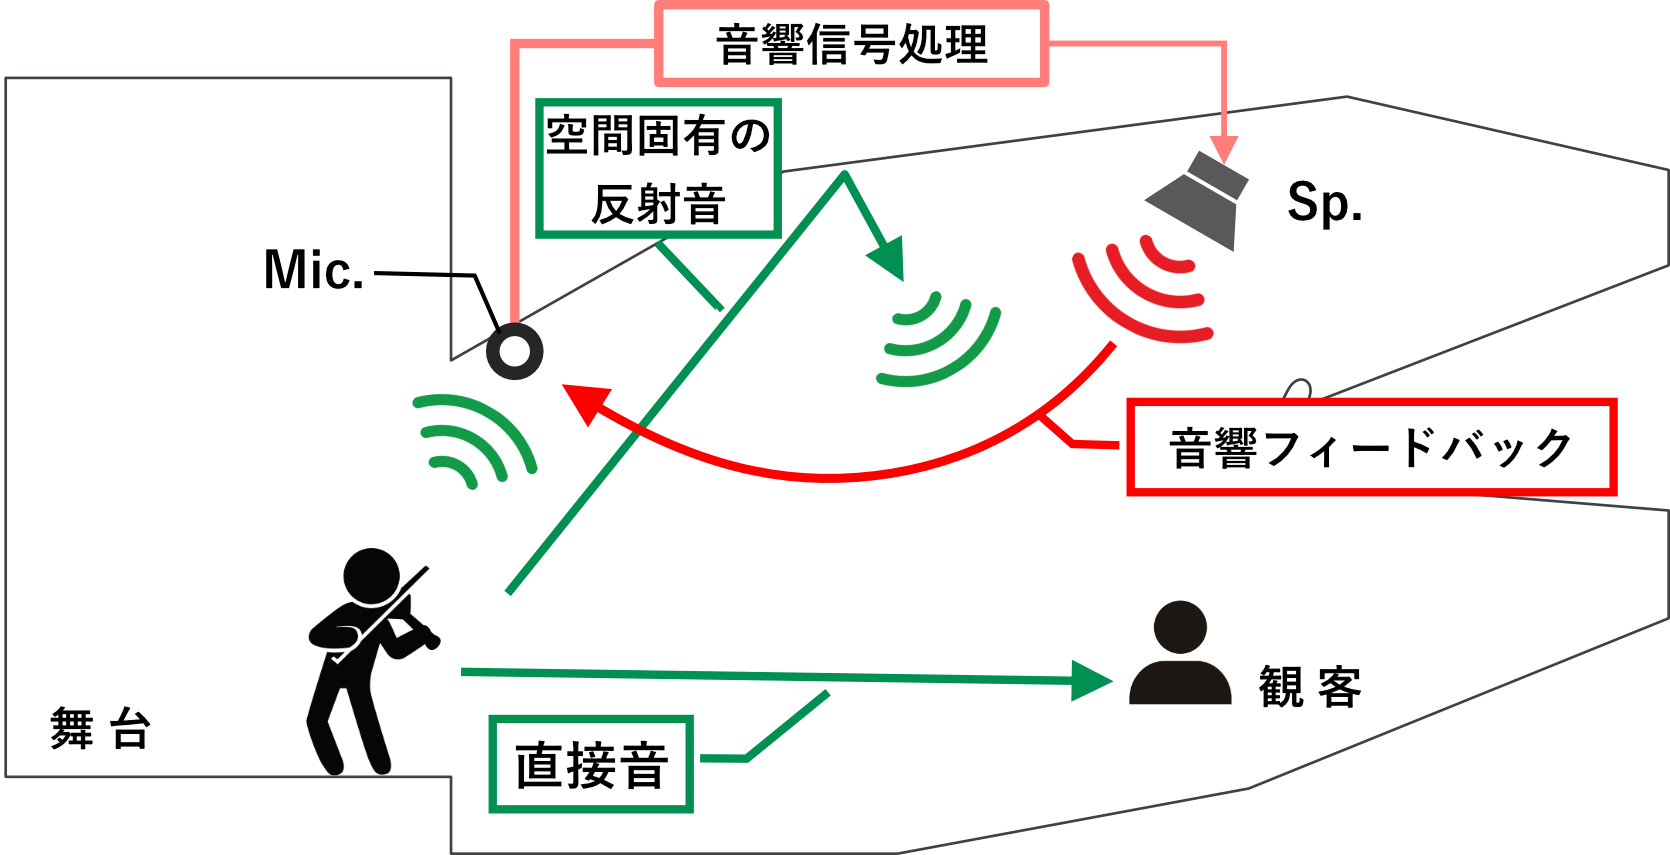
\includegraphics[width=.8\linewidth]{images/afcBasicConcept.png}
  \caption{AFCシステムの基本コンセプト}
  \label{fig:AFCシステムの基本コンセプト}
\end{figure}

\begin{figure}[H]
  \begin{minipage}[t]{0.5\linewidth}
    \centering
    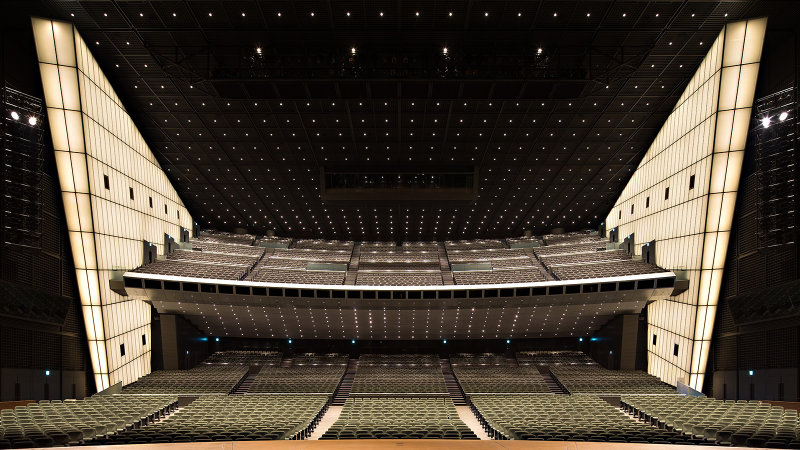
\includegraphics[width=0.9\linewidth]{images/pictureCitation/resized/tokyoForum.jpg}
    \caption{東京国際フォーラム ホールA}
    \footnotesize 東京国際フォーラム公式ホームページより引用 \cite{tokyoForum}
    \label{fig:東京国際フォーラム}
  \end{minipage}%
  \begin{minipage}[t]{0.5\linewidth}
    \centering
    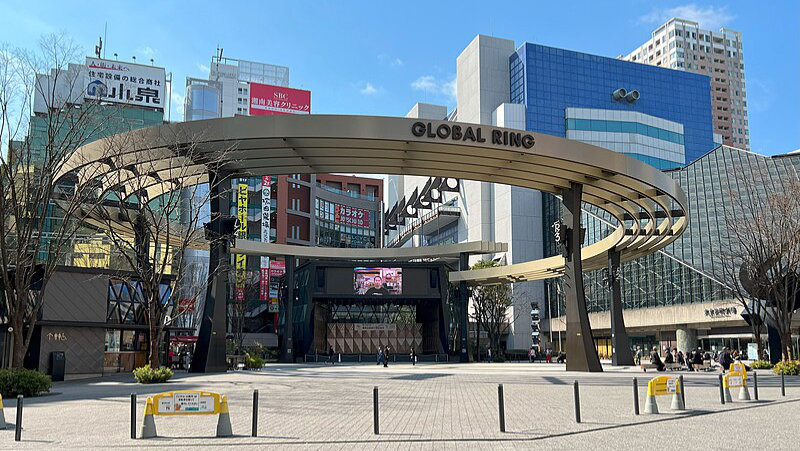
\includegraphics[width=0.9\linewidth]{images/pictureCitation/resized/globalRing.jpg}
    \caption{池袋西口公園 グローバルリングシアター}
    \label{fig:グローバルリングシアター}
    \footnotesize © Asanagi Wikipediaより引用 \cite{globalRing}
  \end{minipage}
\end{figure}

\vspace{\stretch{1}}

%=======================================================================
\newpage
\section{本論文の構成} %1.5
本論文は全5章から構成される。

第1章では、研究の背景としてコンサートホールとその研究について概観し、コンサートホール音響学の一領域であるステージ音響学と、特に反射音の方向特性に関する既往研究について整理した。さらに、本研究の目的として反射音到来方向が演奏者に与える影響について検討することを述べ、また本研究で用いる実験システムであるAFCについて簡単に紹介した。

第2章では、反射音の到来方向について物理的に評価する方法の提案を行い、その方法によって実際のコンサートホールにおける反射音到来方向特性を評価し、その結果を考察する。さらに、それを踏まえて、演奏実験を行うための生成音場の目標値を設定する。

第3章では、第2章では、本研究で用いる音場生成システムであるAFCの仕組み、およびそれを導入した実験室のシステム機器構成について説明し、AFCを用いた音場の生成方法と生成された音場の音響特性について述べる。

第4章では、第3章で得られた音場を用いて行った演奏実験について、その方法、結果および考察について述べる。

第5章では、本研究で得られた成果を整理して総括し、今後の課題と展望について述べる。

\cleardoublepage

% 参考文献
% 参考文献の箇所にインプットしてください。

% 分割ファイル内でのみ,bibliographyを読み込みます。

\expandafter\ifx\csname ifdraft\endcsname\relax

  % bibliographyを展開する

  \bibliographystyle{junsrt}
  \bibliography{ref.bib}% 同じディレクトリ内のbibファイルのみを参照可能

\fi

\end{document}